\documentclass[twocolumn, a4paper]{article}
\usepackage[a4paper, left = 2cm, right = 2cm, top = 2cm, bottom = 2cm]{geometry}
\usepackage[style = numeric, sorting = none, urldate = long]{biblatex}
\usepackage{subfig}
\usepackage{pgfplots}
\usepackage[T1]{fontenc}
\usepackage{graphicx}

\graphicspath{{./images/}}
\addbibresource{refs.bib}

\renewcommand*{\bibfont}{\footnotesize}

\author{
    George Herbert\\
    \texttt{cj19328@bristol.ac.uk}
}

\title{\vspace{-2em}Optimising and Parallelising d2q9-bgk.c}
\begin{document}

\maketitle

\begin{abstract}
    \texttt{d2q9-bgk.c} implements the Lattice Boltzmann method (LBM) to simulate a fluid density on a lattice.
    This report outlines the techniques I utilised to optimise and parallelise \texttt{d2q9-bgk.c} and a detailed analysis of those techniques.
\end{abstract}

\section{Original Code}

I ran the provided \texttt{Makefile} to compile the original \texttt{d2q9-bgk.c} code, which executed the GNU Compiler Collection (GCC) with the \texttt{-std=c99} \texttt{-O3} and \texttt{-lm} options.
Table \ref{tab:original} contains the execution time for each test case.

\begin{table}[htbp]
    \begin{center}
    \caption{Execution times of the original code}\label{tab:original}
    \begin{tabular}{l | l} 
        \hline\hline
        Grid Size&Time (s)\\
        \hline
        $128 \times 128$&\texttt{ 29.16}\\
        $128 \times 256$&\texttt{ 58.71}\\
        $256 \times 256$&\texttt{233.32}\\
        $1024 \times 1024$&\texttt{980.89}\\
        \hline
      \end{tabular}
    \end{center}
\end{table} 

I measured the original code to quantify the performance improvements of my latter implementations.
Each time is an average of five runs on BlueCrystal Phase 4's (BC4's) compute nodes; each of which was a Lenovo nx360 M5, which contained two 14-core 2.4 GHz Intel E5-2680 v4 (Broadwell) CPUs and 128 GiB of RAM \cite{bcp4}.
I took an average because of the variation between runs, which existed due to the inconsistent performance of compute nodes.
% Not all compute nodes offer the same performance all of the time, due to differing placement in the data centre, amongst other reasons.

\section{Compiler Optimisations}

% I initially implemented a collection of serial optimisations to improve the performance of \texttt{d2q9-bgk.c}.

\subsection{Intel C Compiler Classic}

I hypothesised that compiling with the Intel C Compiler Classic (ICC) instead of GCC would produce an executable better optimised for BC4's Intel compute nodes.
Table \ref{tab:icc} contains the execution times after compiling with ICC.

\begin{table}[htbp]
  \begin{center}
  \caption{Execution times using ICC and speedup over the prior implementation}\label{tab:icc}
  \begin{tabular}{l | l l} 
      \hline\hline
      Grid Size&Time (s)&Speedup\\
      \hline
      $128 \times 128$&\texttt{}&\texttt{}\\
      $128 \times 256$&\texttt{}&\texttt{}\\
      $256 \times 256$&\texttt{}&\texttt{}\\
      $1024 \times 1024$&\texttt{}&\texttt{}\\
      \hline
    \end{tabular}
  \end{center}
\end{table}

\subsection{Compiler Options}

I hypothesised that I could compile my program with more aggressive optimisations to improve performance, whilst still producing the correct solution.
I compiled my code with the \texttt{-Ofast} option, which implemented additional aggressive floating-point optimisations \cite{icc}.
These changes to the compilation process provided a good performance boost, as evident in Table \ref{tab:compiler_options}.

\begin{table}[htbp]
  \begin{center}
  \caption{Execution times using new ICC options and speedup over the prior implementation}\label{tab:compiler_options}
  \begin{tabular}{l | l l} 
      \hline\hline
      Grid Size&Time (s)&Speedup\\
      \hline
      $128 \times 128$&\texttt{ 22.25}&\texttt{}\\
      $128 \times 256$&\texttt{ 44.42}&\texttt{}\\
      $256 \times 256$&\texttt{176.69}&\texttt{}\\
      $1024 \times 1024$&\texttt{795.41}&\texttt{}\\
      \hline
    \end{tabular}
  \end{center}
\end{table}

\section{Serial Optimisations}

I used the Intel Advisor tool to generate a Roofline chart, as shown in Figure \ref{fig:roofline_compiler}.

\begin{figure}[htbp]
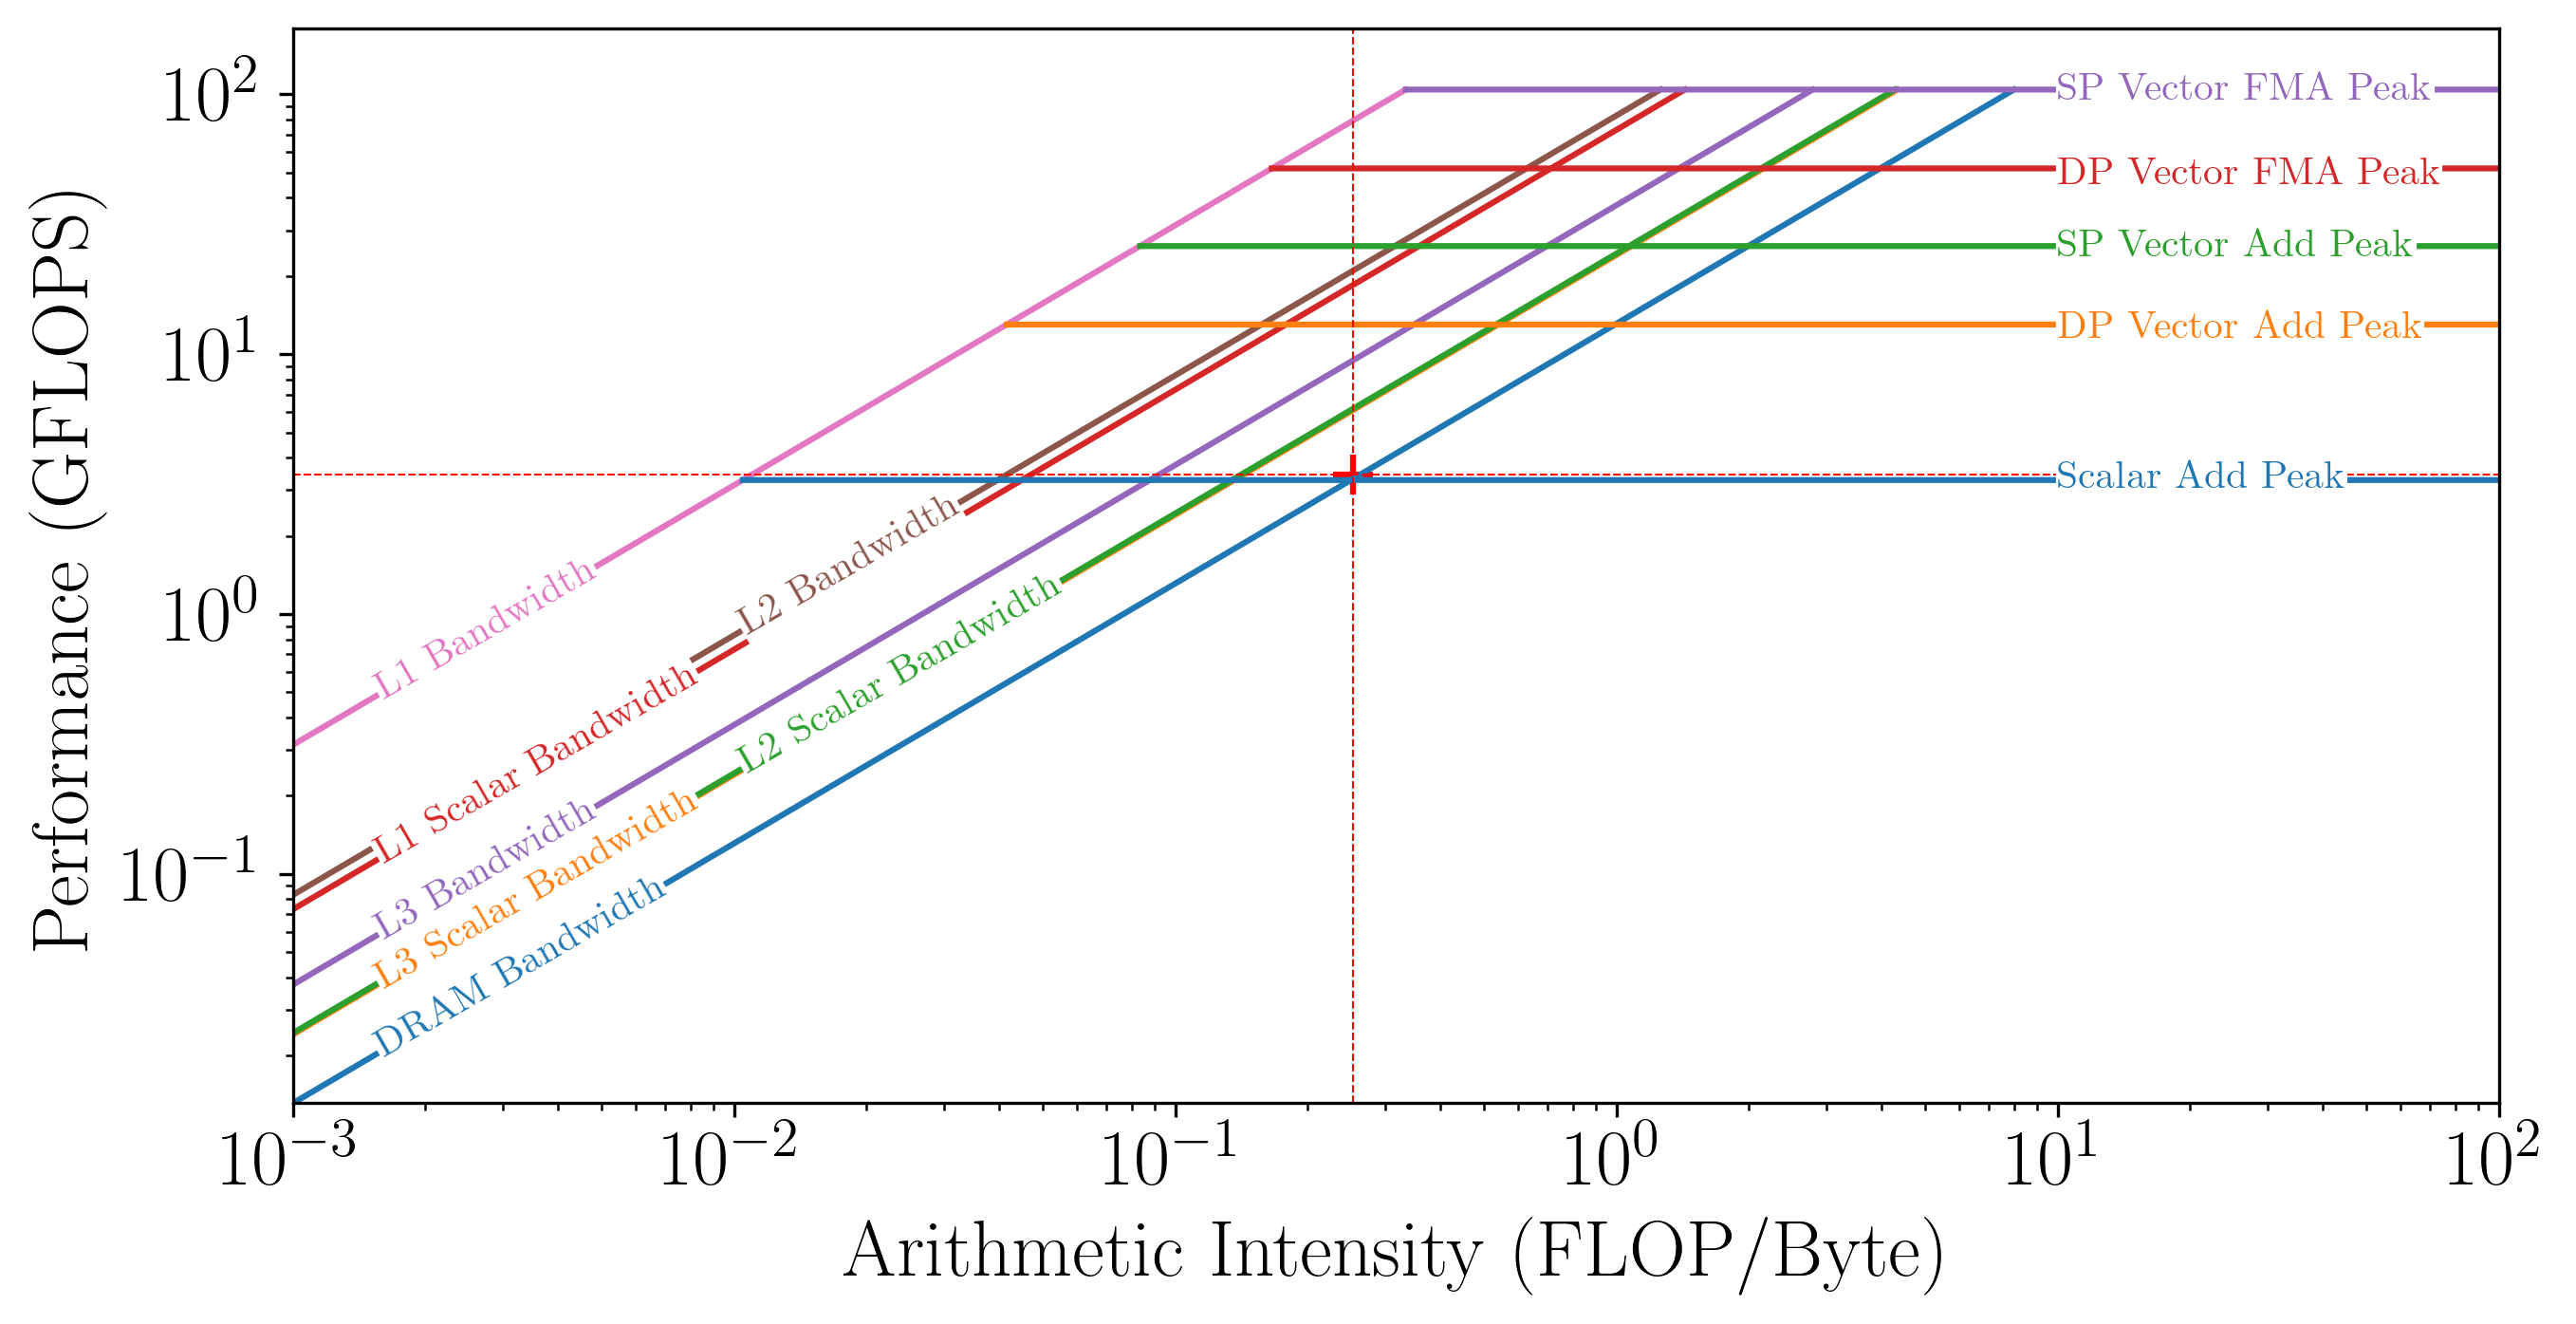
\includegraphics[width=\linewidth]{roofline_compiler.png}
\caption{Screenshot of the Roofline chart following compilation changes, run on the $1024\times1024$ test case}\label{fig:roofline_compiler}
\end{figure}

I identified several attributes of my program and several key areas to focus my optimisations.
For larger grid sizes especially, the LBM implementation in \texttt{d2q9-bgk.c} was a memory bandwidth bound problem.
\texttt{d2q9-bgk.c} achieved an average arithmetic intensity of 0.25 FLOP/byte and performance of 3.44 GFLOPS for the $1024 \times 1024$ test case.

\subsection{Loop Fusion}

Using the Roofline chart, I identified that decreasing the number of accesses to memory within each timestep would simultaneously increase my program's performance whilst also increasing the arithmetic intensity, thus raising the performance bound for my latter implementations. 

To accomplish this I implemented loop fusion.
In the original code, the entire grid was iterated over in four sequential procedures within each timestep: \texttt{propagate}, \texttt{rebound}, \texttt{collision} and \texttt{av\_velocity}.
I fused the four loops within these procedures into a single loop in the \texttt{timestep} procedure.
This enabled me to eliminate the temporary allocations of cell values to the \texttt{tmp\_cells} array.
Instead, all new values of cells are written to the \texttt{cells\_new} array, and the pointers of \texttt{cells} and \texttt{cells\_new} are swapped each timestep.

Table \ref{tab:loop_fusion_pointer_swap} displays the improvements to the execution time.
Moreover, my program's arithmetic intensity increased to 0.29 FLOP/byte, and the performance increased to 3.54 GFLOPS for the $1024 \times 1024$ test case.

\begin{table}[htbp]
  \begin{center}
  \caption{Execution times with loop fusion and pointer swap, and speedup over the prior implementation}\label{tab:loop_fusion_pointer_swap}
  \begin{tabular}{l | l l} 
      \hline\hline
      Grid Size&Time (s)&Speedup\\
      \hline
      $128 \times 128$&\texttt{ 19.42}&\texttt{1.15}\\
      $128 \times 256$&\texttt{ 39.21}&\texttt{1.13}\\
      $256 \times 256$&\texttt{155.64}&\texttt{1.14}\\
      $1024 \times 1024$&\texttt{635.61}&\texttt{1.25}\\
      \hline
    \end{tabular}
  \end{center}
\end{table}

\subsection{Arithmetic}

Despite the compiler optimising the arithmetic within each timestep, I hypothesised I could make some manual improvements to further reduce my program's execution time.

Division operations take considerably more time to execute than other basic arithmetic operations, such as multiplication.
To eliminate a several unnecessary division operations, I precalculated several values: \texttt{c\_sq\_r}, the reciprocal of $c^2$; \texttt{two\_c\_sq\_r}, the reciprocal of $2c^2$; and \texttt{two\_c\_sq\_sq\_r}, the reciprocal of $2c^4$, where $c$ is the speed of sound.
I then replaced several division operations with multiplications by these values.

Additionally, I eliminated the repeated calculation and division of \texttt{tot\_cells} (i.e. the number of cells that were not obstacles) each timestep.
To do so, my program calculated \texttt{tot\_cells} once during the initialisation phase.
I then set the reciprocal of this value in the \texttt{params.num\_non\_obstacles\_r} variable, which I multiplied with \texttt{tot\_u} to compute the average velocity each timestep.

These arithmetic improvements provided only a slight speedup compared to the prior implementation, as shown in Table \ref{tab:arithmetic_improvements}.
This was because the execution time of my program was dominated by memory accesses.
I would expect a larger speedup in smaller grid sizes than the test cases provided.

\begin{table}[htbp]
  \begin{center}
  \caption{Execution times with arithmetic improvements and speedup over the prior implementation}\label{tab:arithmetic_improvements}
  \begin{tabular}{l | l l} 
      \hline\hline
      Grid Size&Time (s)&Speedup\\
      \hline
      $128 \times 128$&\texttt{ 19.10}&\texttt{1.02}\\
      $128 \times 256$&\texttt{ 38.49}&\texttt{1.02}\\
      $256 \times 256$&\texttt{153.39}&\texttt{1.01}\\
      $1024 \times 1024$&\texttt{621.52}&\texttt{1.02}\\
      \hline
    \end{tabular}
  \end{center}
\end{table}

\section{Vectorization}

Vectorization is the process of converting a scalar implementation to a vector implementation, which enables the compiler to use additional registers to perform single, multiple data (SIMD) operations.

\subsection{Structure of Arrays}

I hypothesised that converting the \texttt{t\_speed} structrue from an array of structures (AoS) to a structure of arrays (SoA) would suit vectorisation of the inner loop; the SoA format would keep memory accesses contiguous over structure instances.
I altered the \texttt{t\_speed} to contain nine pointers, each to an individual array of floats.
Each array of floats contained the values of one vector for each cell within the grid.

The SoA format actually increased the execution time of my program, as shown in Table \ref{tab:soa}.
This is because the AoS format has better memory locality in the program's unvectorized form.

\begin{table}[htbp]
  \begin{center}
  \caption{Execution times with SoA and speedup over the prior implementation}\label{tab:soa}
  \begin{tabular}{l | l l} 
      \hline\hline
      Grid Size&Time (s)&Speedup\\
      \hline
      $128 \times 128$&\texttt{}&\texttt{}\\
      $128 \times 256$&\texttt{}&\texttt{}\\
      $256 \times 256$&\texttt{}&\texttt{}\\
      $1024 \times 1024$&\texttt{}&\texttt{}\\
      \hline
    \end{tabular}
  \end{center}
\end{table}

\subsection{Memory Alignment and Disambiguation}

Processors efficiently move data located on specific byte boundaries by the nature of their design, and compilers can perform optimisations when data access is known to be aligned by 64 bytes \cite{alignment}.
To align the \texttt{cells}, \texttt{cells\_new} and \texttt{obstacles} variables, I replaced calls to the \texttt{malloc} and \texttt{free} procedures with the alignment specific replacements: \texttt{\_mm\_malloc} and \texttt{\_mm\_free}, respectively.
I used the \texttt{\_\_assume\_\_aligned} procedure and  the statement \texttt{\_\_assume(params.nx \% 16 == 0)} to inform the compiler that the dynamically allocated variables were aligned.
Doing so prevented the compiler from generating conservative code, which would have been detrimental to the speed of my implementation.

I compiled my code with the \texttt{-restrict} option and used the \texttt{restrict} keyword to define each of the nine pointers in \texttt{t\_speed}.
The \texttt{restrict} keyword asserted that the memory referenced by these pointers was not aliased.
Overall, this reduced the execution time by preventing the compiler from performing a runtime check for aliasing.

\begin{table}[htbp]
  \begin{center}
  \caption{Execution times with memory improvements and speedup over the prior implementation}\label{tab:memory}
  \begin{tabular}{l | l l} 
      \hline\hline
      Grid Size&Time (s)&Speedup\\
      \hline
      $128 \times 128$&\texttt{}&\texttt{}\\
      $128 \times 256$&\texttt{}&\texttt{}\\
      $256 \times 256$&\texttt{}&\texttt{}\\
      $1024 \times 1024$&\texttt{}&\texttt{}\\
      \hline
    \end{tabular}
  \end{center}
\end{table}

\subsection{SIMD Directives}

Having altered the data layout to suit vectorization, I utilised several other techniques to enforce vectorization.
I implemented the \texttt{\#pragma omp simd} pragma to vectorise the inner loop within each timestep.
This pragma indicated to the compiler to utilise SIMD instructions to execute operations within the inner loop on multiple data elements in a single instruction.
Furthermore, I utilised the \texttt{reduction(+:tot\_u)} clause to ensure the \texttt{tot\_u} variable contained the correct value at the loop's termination.

Once I had utilised these techniques to enforce efficient vectorization of the inner loop, I compiled \texttt{d2q9-bgk.c} with the \texttt{-xAVX2} option to direct the compiler to optimise for Intel processors that support Advanced Vector Extensions 2 (AVX2) (which BC4's compute nodes do) \cite{lenovo}.
I did not have to compile with any additional options to enable the compiler to follow OpenMP SIMD directives since the \texttt{-qopenmp-simd} option was enabled by default at the \texttt{-Ofast} optimisation level \cite{icc}.

Vectorization provided the most considerable improvement to speedup of any optimisation that I had implemented to this point, as shown in Table \ref{tab:vectorized}.
Furthermore, my implementation achieved an arithmetic intensity of 0.43 FLOP/byte and performance of 10.14 GFLOPS when run on the $1024\times1024$ test case.
% This significant improvement was unsurprising since AVX2 could perform simultaneous operations on up to eight single-precision floating-point numbers.

\begin{table}[htbp]
  \begin{center}
  \caption{Execution times with vectorization and speedup over the prior implementation}\label{tab:vectorized}
  \begin{tabular}{l | l l} 
      \hline\hline
      Grid Size&Time (s)&Speedup\\
      \hline
      $128 \times 128$&\texttt{  \,\,\,5.77}&\texttt{}\\
      $128 \times 256$&\texttt{ 11.57}&\texttt{}\\
      $256 \times 256$&\texttt{ 41.55}&\texttt{}\\
      $1024 \times 1024$&\texttt{215.52}&\texttt{}\\
      \hline
    \end{tabular}
  \end{center}
\end{table}

\section{Parallelism}

% Overall, my serial optimisations (including vectorization) achieved approximately five times speedup over the original implementation.
% However, there was an immense potential for performance improvements by parallelising \texttt{d2q9-bgk.c}. 

\subsection{OpenMP}

OpenMP implements parallelism by launching a set of threads that execute portions of code concurrently.
I utilised OpenMP's \texttt{\#pragma omp parallel for} pragma to direct the compiler to parallelise the outer loop in the \texttt{timestep} procedure.
Furthermore, I compiled my code with the \texttt{-qopenmp} option, which enabled the paralleliser to generate multithreaded code based on OpenMP directives.
Since the \texttt{tot\_u} variable needed to contain the total velocities of each cell, I used the clause \texttt{reduction(+:tot\_u)} to prevent race conditions; the reduction clause informed the compiler to create a copy of the \texttt{tot\_u} variable for each thread (initialised to zero), and to sum the local results when the outer loop terminated.

Table \ref{tab:parallelised} displays the execution times for my parallel implementation (run with 28 threads), and speedup over both the original and vectorized code.

\begin{table}[htbp]
  \begin{center}
  \caption{Execution times with 28 threads and speedup over the prior implementation}\label{tab:parallelised}
  \begin{tabular}{l | l l} 
      \hline\hline
      Grid Size&Time (s)&Speedup\\
      \hline
      $128 \times 128$&\texttt{ 1.14}&\texttt{5.05}\\
      $128 \times 256$&\texttt{ 1.35}&\texttt{5.07}\\
      $256 \times 256$&\texttt{ 3.33}&\texttt{5.62}\\
      $1024 \times 1024$&\texttt{14.38}&\texttt{4.55}\\
      \hline
    \end{tabular}
  \end{center}
\end{table}

\subsection{Non-Uniform Memory Access (NUMA)}

NUMA is a computer memory design in which memory access time depends on the memory location relative to the processor.
Memory is allocated to the closest NUMA region to the thread that first touches the data.
Since BC4's compute nodes contain two sockets, the memory access time for a given thread primarily depends on whether the memory is connected to the socket the thread resides in or not.
As a result, I parallelised the initialisation loops for \texttt{cells} and \texttt{obstacles} to ensure that each thread touched the same data in both the \texttt{initialise} and \texttt{compute} procedures.
Furthermore, I set the environment variables \texttt{OMP\_PROC\_BIND=true} and \texttt{OMP\_PLACES=cores} to prevent threads from moving cores.

Table \ref{tab:numa} contains the updated execution times for my final NUMA-aware implementation.

\begin{table}[htbp]
  \begin{center}
  \caption{Execution times with NUMA-aware 28 threads and speedup over the prior implementation}\label{tab:numa}
  \begin{tabular}{l | l  l  l} 
      \hline\hline
      &&\multicolumn{2}{c}{Speedup}\\
      \cline{3-4}
      Grid Size&Time (s)&Original&Vectorized\\
      \hline
      $128 \times 128$&\texttt{ 0.72}&\texttt{}&\texttt{ 8.01}\\
      $128 \times 256$&\texttt{ 0.80}&\texttt{}&\texttt{14.46}\\
      $256 \times 256$&\texttt{ 2.47}&\texttt{}&\texttt{16.82}\\
      $1024 \times 1024$&\texttt{12.81}&\texttt{}&\texttt{16.83}\\
      \hline
    \end{tabular}
  \end{center}
\end{table}

\subsection{Scaling}

I ran my final, NUMA-aware implementation on one to 28 threads to gain an insight into how my implementation scaled.
I calculated the speedup that subsequent threads provided over a single thread implementation.
Figure \ref{fig:scaling} displays the resultant speedup curves.

\begin{figure}[htpb]
  \centering
  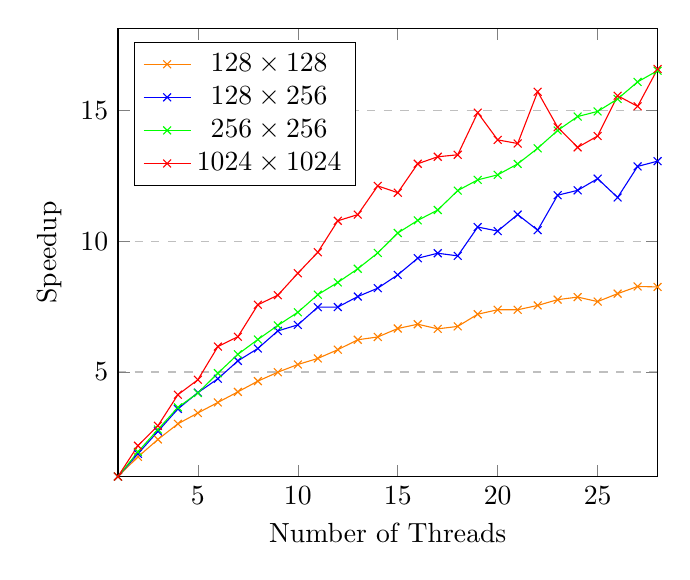
\begin{tikzpicture}
    \begin{axis}[
      xlabel={Number of Threads},
      ylabel={Speedup},
      xmin = 1, xmax = 28,
      ymin = 1,
      % xtick={0, 5, 10, 15, 20, 25},
      % ytick={0,20,40,60,80,100,120},
      legend pos=north west,
      ymajorgrids=true,
      grid style=dashed,
    ]
    \addlegendentry{$128\times128$}
    \addplot[color = orange, mark = x]coordinates{
      (1, 1.0)
      (2, 1.7525169788462858)
      (3, 2.419897249840069)
      (4, 3.0177321760395954)
      (5, 3.4340474353625594)
      (6, 3.8362657949346852)
      (7, 4.241072726461517)
      (8, 4.651864978037027)
      (9, 4.993654422331282)
      (10,5.2882280154084835)
      (11,5.520195387872089)
      (12,5.854579031493787)
      (13,6.23457059163917)
      (14,6.342501046595846)
      (15,6.666023078680611)
      (16,6.829810732132427)
      (17,6.6526516481296065)
      (18,6.746204776109836)
      (19,7.213003419569139)
      (20,7.383978810814603)
      (21,7.383266518002555)
      (22,7.548589923892521)
      (23,7.770076587082373)
      (24,7.86829502746941)
      (25,7.69660960948019)
      (26,8.000150678051229)
      (27,8.274732001825265)
      (28,8.256913368882064)
    };
    \addlegendentry{$128\times256$}
    \addplot[color = blue, mark = x]coordinates{
      (1, 1)
      (2, 1.87192962)
      (3, 2.728614279)
      (4, 3.588436108)
      (5, 4.211061907)
      (6, 4.74277418)
      (7, 5.426597365)
      (8, 5.901009271)
      (9, 6.574136151)
      (10,6.804566205)
      (11,7.483065988)
      (12,7.486914766)
      (13,7.888917429)
      (14,8.209594871)
      (15,8.719464845)
      (16,9.356809194)
      (17,9.546299879)
      (18,9.445666983)
      (19,10.54931431)
      (20,10.3964243)
      (21,11.02717878)
      (22,10.42891424)
      (23,11.76705845)
      (24,11.95396706)
      (25,12.40123763)
      (26,11.68112555)
      (27,12.86943567)
      (28,13.07066895)
    };
    \addlegendentry{$256\times256$}
    \addplot[color = green, mark = x]coordinates{
      (1, 1)
      (2, 1.945477182)
      (3, 2.800216561)
      (4, 3.646333662)
      (5, 4.198400745)
      (6, 4.956879242)
      (7, 5.677667438)
      (8, 6.245197272)
      (9, 6.784427958)
      (10,7.287431021)
      (11,7.959683682)
      (12,8.429533225)
      (13,8.952220823)
      (14,9.559358953)
      (15,10.32030432)
      (16,10.80402701)
      (17,11.20107215)
      (18,11.94368597)
      (19,12.3549946)
      (20,12.54738718)
      (21,12.96564369)
      (22,13.56433482)
      (23,14.24616986)
      (24,14.77874954)
      (25,14.97434191)
      (26,15.45192009)
      (27,16.10441691)
      (28,16.53368092)

    };
    \addlegendentry{$1024\times1024$}
    \addplot[color = red, mark = x]coordinates{
      (1, 1)
      (2, 2.182054561)
      (3, 2.943754524)
      (4, 4.131667716)
      (5, 4.705750019)
      (6, 5.973656817)
      (7, 6.351981192)
      (8, 7.573833461)
      (9, 7.941396106)
      (10,8.7813412)
      (11,9.58468842)
      (12,10.78916878)
      (13,11.02458512)
      (14,12.12324785)
      (15,11.86351157)
      (16,12.97218687)
      (17,13.23885542)
      (18,13.31481491)
      (19,14.92644603)
      (20,13.88484436)
      (21,13.74639988)
      (22,15.72695273)
      (23,14.36825215)
      (24,13.59839996)
      (25,14.03417467)
      (26,15.5747082)
      (27,15.16956075)
      (28,16.59876059)
    };
    \end{axis}
  \end{tikzpicture}
  \caption{Speedup curves for my NUMA-aware implementation}\label{fig:scaling}
\end{figure}

In general, my implementation initially scaled well for each grid size, but the speedup acquired from each subsequent thread declines---this is known as a sublinear plateau.
Notably, the amount of speedup provided by each subsequent core is approximately inversely proportional to the test case size.
In other words, larger grid sizes benefit more from a multithreaded implementation than smaller grid sizes---this is because the smaller grids saturate the memory bandwidth sooner.

\subsection{Comparison to Serial Optimised}

I used the Intel Advisor tool to analyse the performance of my final implementation, as shown in Figure \ref{fig:roofline_numa}.
On the $1024\times1024$ test case, my program achieved an arithmetic intensity of 0.43 FLOP/byte and 168.35 GFLOPS of performance.

\begin{figure}[htbp]
  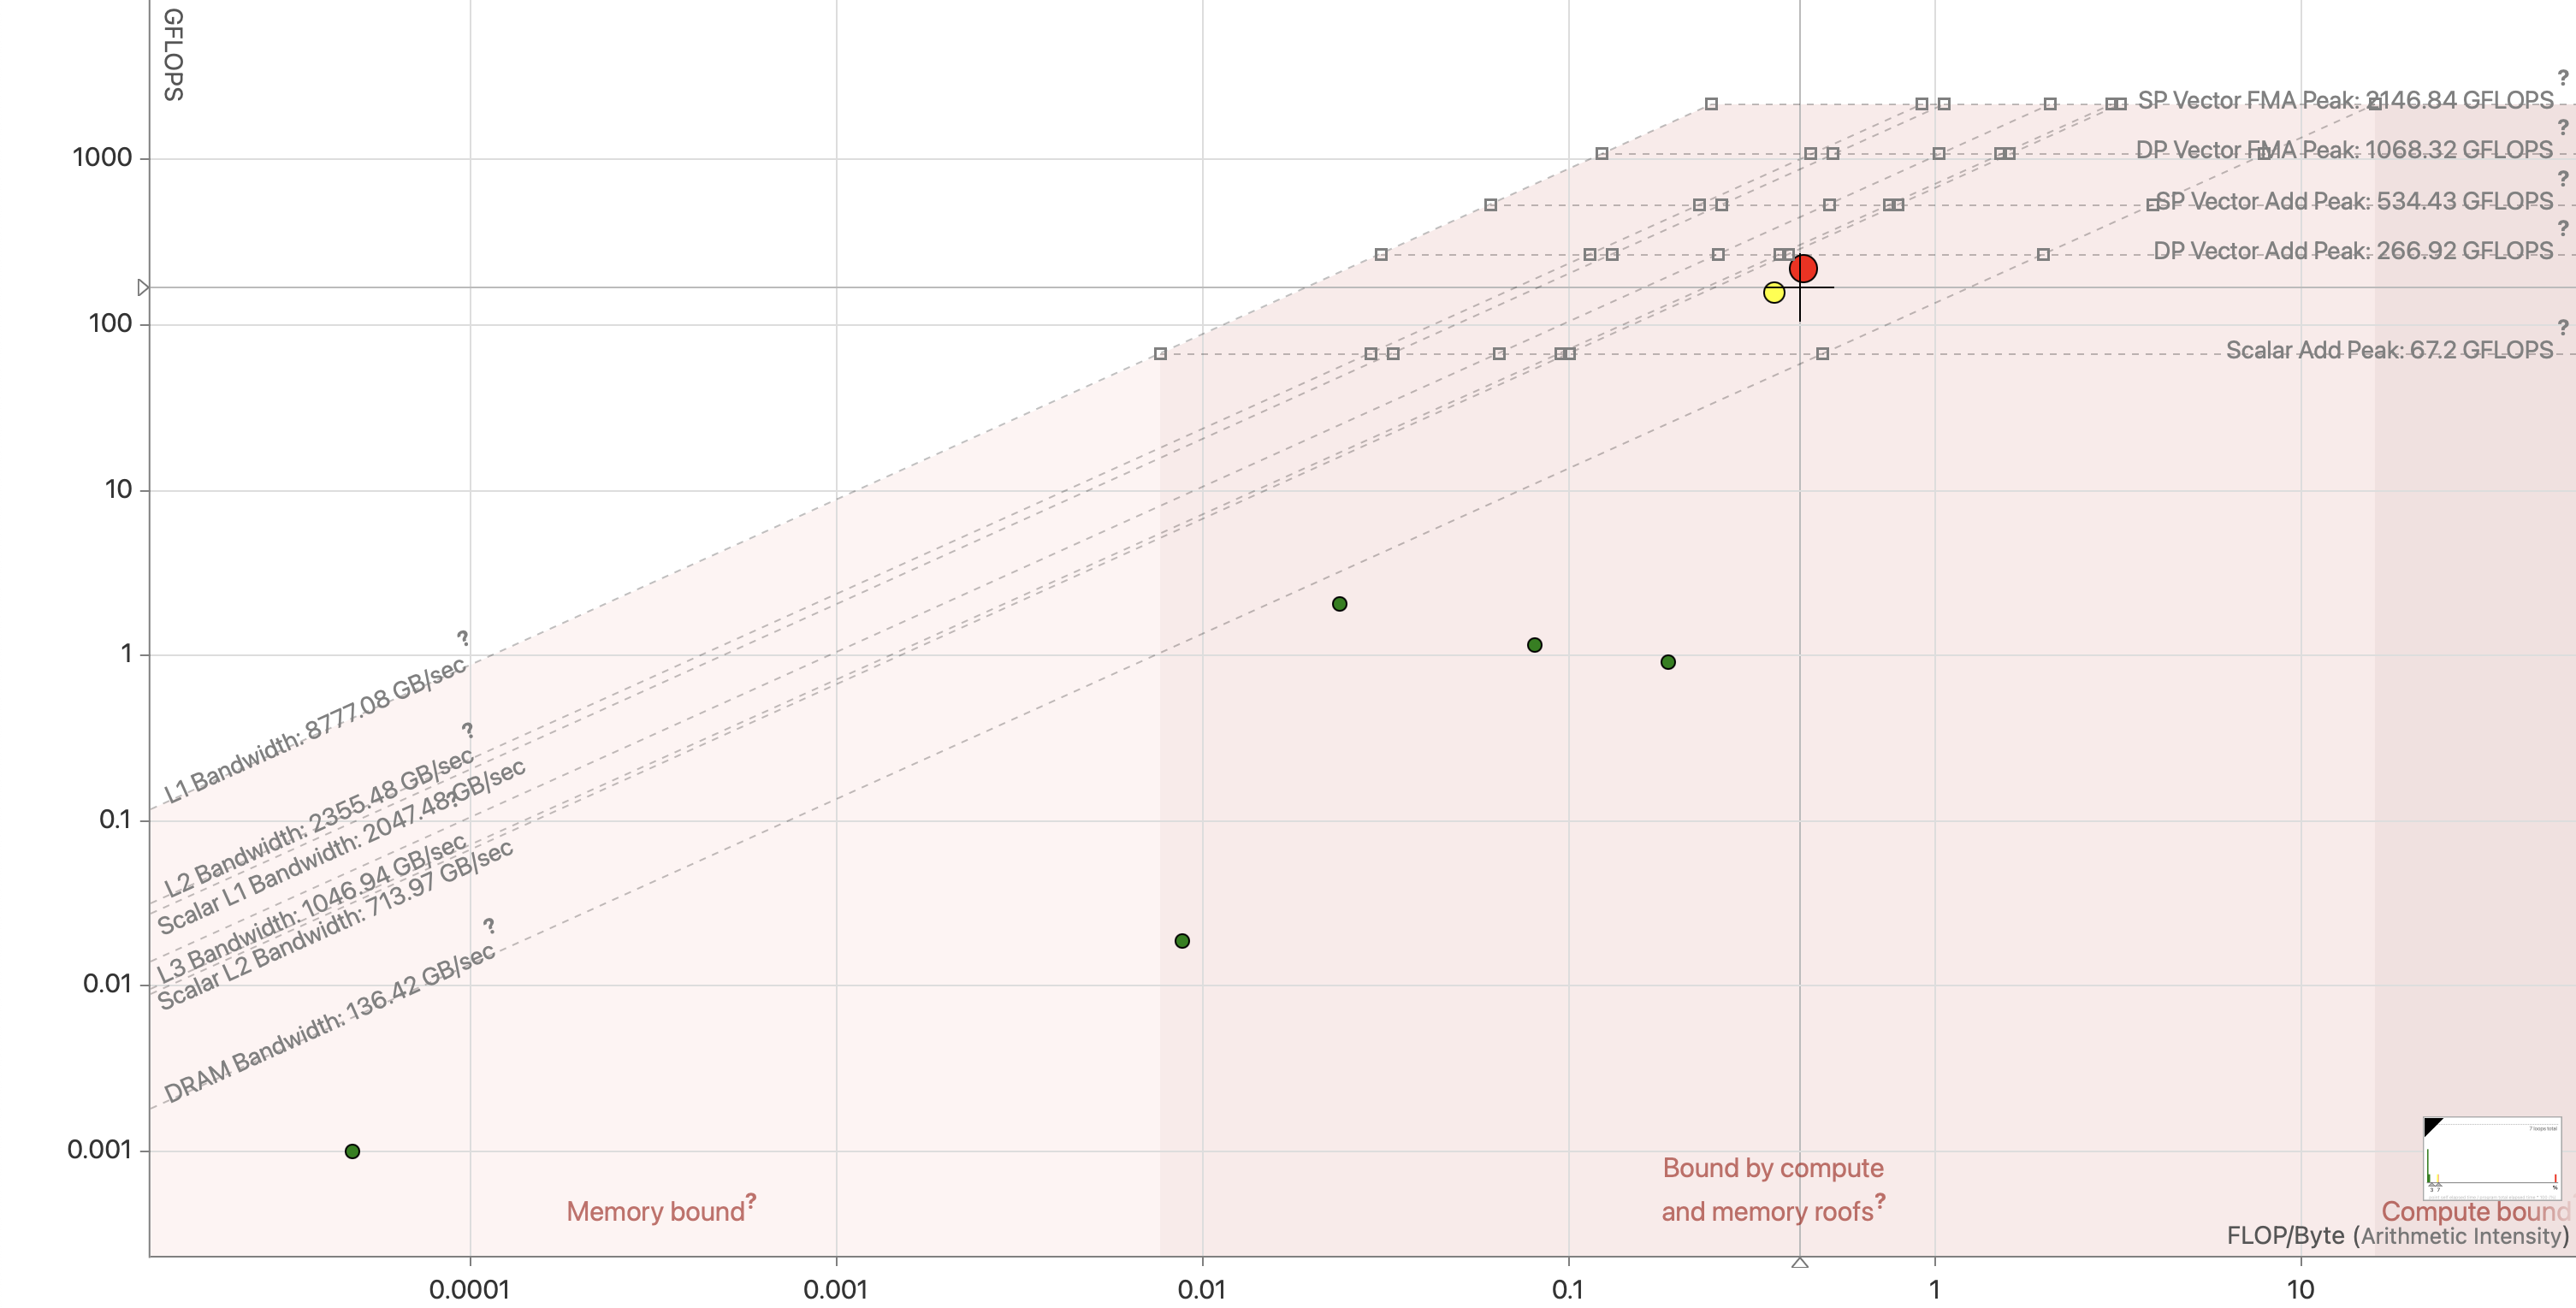
\includegraphics[width=\linewidth]{roofline_numa.png}
  \caption{Screenshot of the Intel Advisor Roofline Analysis for my NUMA-aware implementation, run with 28 threads on the $1024\times1024$ test case}\label{fig:roofline_numa}
\end{figure}

Compared to my vectorized implementation, the arithmetic intensity was identical, whereas the performance increased by a factor of 16.60.
This was primarily due to two reasons.
Firstly, by running across multiple threads on multiple cores, sections of the grid could be computed in parallel.
Secondly, inspecting the Intel Advisor memory metrics for the $1024\times1024$ grid size highlighted that the parallel program did not have to interact with the DRAM, which had a lower bandwidth, as often.
For example, in the \texttt{timestep} loop in the vectorized implementation, 5130.56 GB and 2306.03 GB of data were passed through the L1 cache and DRAM, respectively.
Whereas in the NUMA-aware implementation, 5777.32 GB and 1447.21 GB of data were passed through the L1 cache and DRAM, respectively. 

\section{LBM in Go}

Many other languages, APIs, and libraries can be utilized to implement LBM; all have associated advantages and disadvantages.

Unlike C, Go is a language with concurrency built into its core design.
Consequently, one can achieve parallelism in Go effortlessly, without requiring significant knowledge of the underlying system or APIs such as OpenMP.
As a final, interesting experiment, I produced an implementation of LBM in Go to identify whether Go's easily-understood core features could achieve a comparable amount of performance.

In experiments, the Go implementation was between seven and sixteen times slower.
Specifically, it achieved a time of 7.66 seconds, 13.10 seconds, 41.83 seconds and 103.02 seconds on the increasingly large test cases.
Upon inspection, there were likely several reasons for the comparatively poor performance.
Firstly, Go's compiler did not perform many optimisations.
Compiling with GCCGO or GOLLVM may have produced a better-optimised executable; however, these required a complicated installation process, which was directly contradictory to the desired simplicity for the experiment.
Secondly, and perhaps most prominently, was the lack of vectorization.
Vectorizing code in Go requires external libraries or assembly, which similarly conflicted with the desired simplicity.

In conclusion, a similar implementation built with Go's easily-understood core features could not achieve an even remotely comparable level of performance.

\printbibliography

\end{document}